\chapter{Design} 

In order to bridge the information gap regarding home energy systems, this study aims to provide households with knowledge of available technologies in the market. 
Based on the findings from pre-study and to address the potential issue of information overload, the study proposes a home energy system recommender to present households with a tailored selection of technologies that better fit their unique home situations. 
For instance, by learning the location of the house, in order to estimate the amount of sunlight it is likely to receive over the course of a year, to evaluate whether installing a \gls{pv} system would be a viable and economic way for the household.
The learning theory suggests that individuals learn new knowledge by connecting it with existing knowledge and experiences, as this helps to create a framework for understanding and retention of the new information.
Therefore, by focusing on personalised recommendations, the study hypothesises that households may be more receptive to learning about home energy technologies. 
Meanwhile, nudging house owners towards making informed decisions. 


\section{Design concept: The home energy system recommender}

The home energy system recommender is a software application that integrates the FLEX models,
offering personalised recommendations to households based on their individual circumstances.
Through the recommended technology configurations and simulated energy costs, 
users will not only be guided on these technologies but also be educated on the potential benefits of transitioning to more sustainable energy systems. 


\section{Input to the recommender}


\subsection{Household profiles}

The concept of household profile has been developed to gain insights into the energy demand and supply dynamics of households. 
To ensure the accuracy of this profile, thereby accurately anticipate household's energy costs, 
various factors that may impact the household's energy consumption must be considered, 4 categories as shown in Figure \ref{fig:profile}, they are 
\emph{the external environment, building materials, energy consumption behaviors, and the current home energy system.}
By creating such a profile, a comprehensive understanding of the household's situation can be attained, enabling the offering of more tailored and effective recommendations.
\begin{figure}[h]
  \centering
  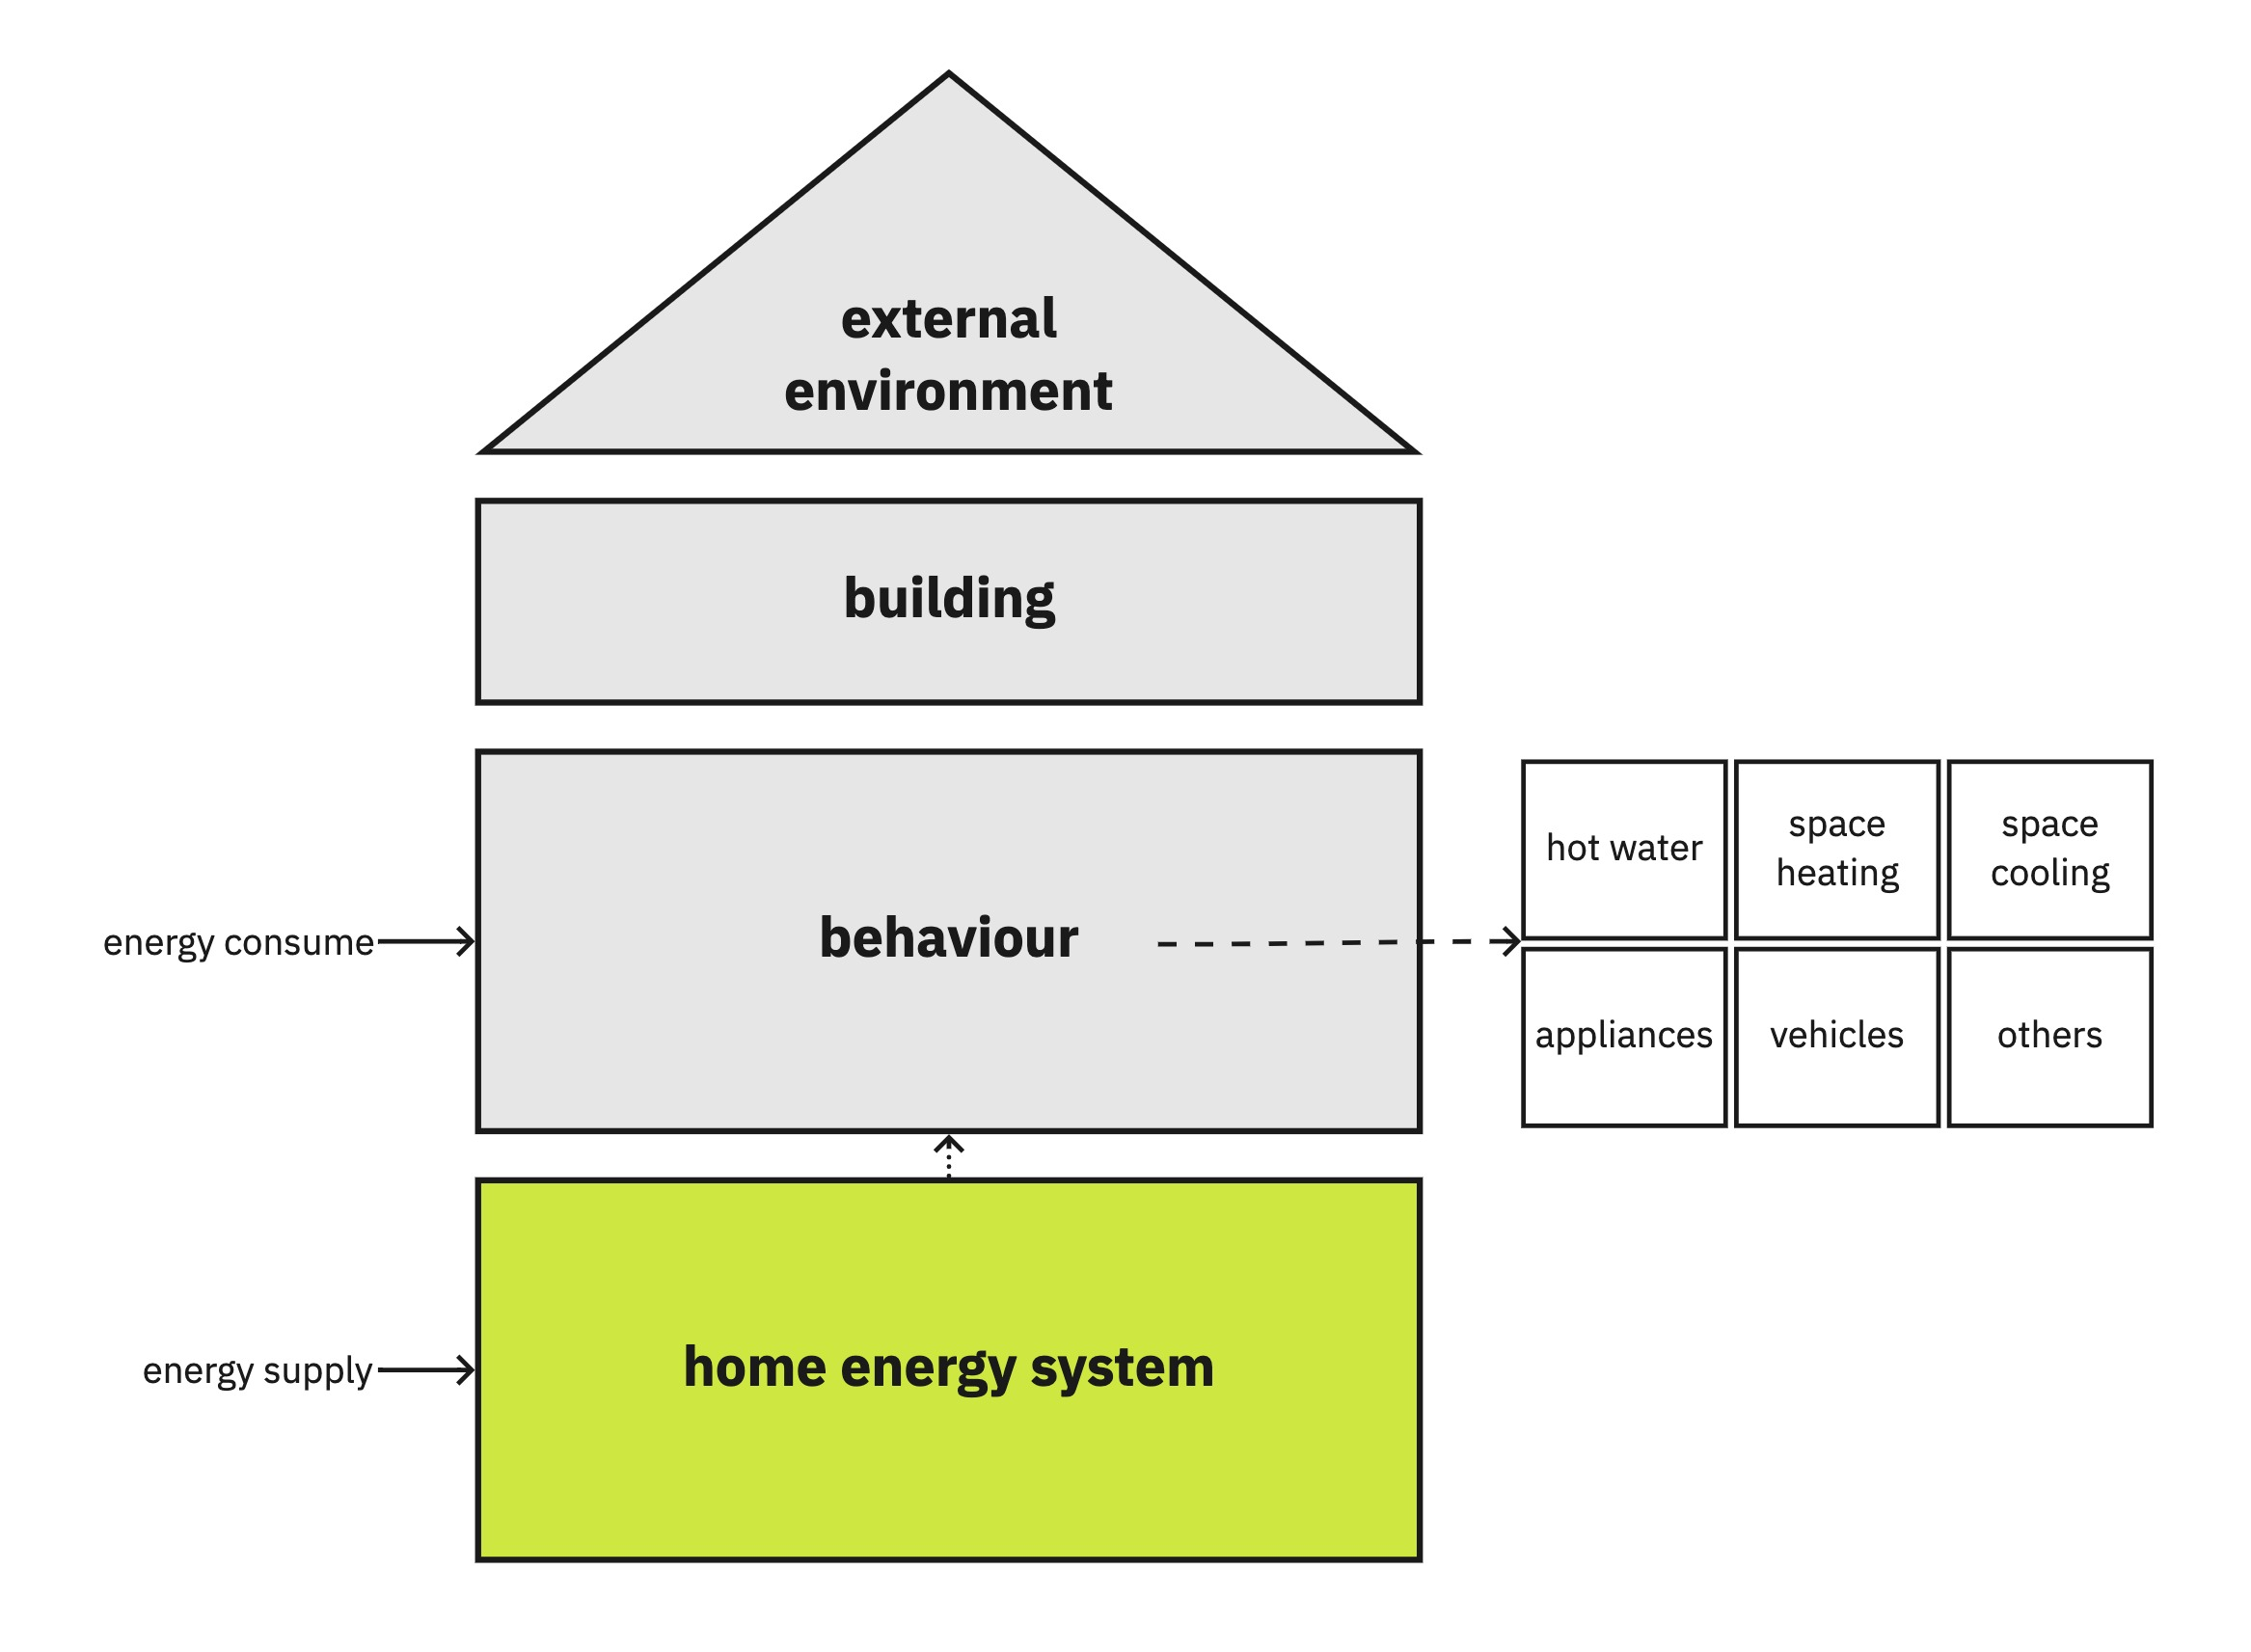
\includegraphics[width=0.4\textwidth]{Images/household_profile.jpg}
  \caption{Household profile}
  \label{fig:profile}
\end{figure}

The categories were inspired by the FLEX models \cite{newtrends}.
The models take a set of variables into account when simulating, they can be divided into following 15 categories: 
\emph{
    behaviour profile,
    battery,
    behaviour, 
    boiler,
    building,
    energy price,
    heating element, 
    hot water tank,
    \gls{pv},
    region,
    space cooling technology,
    space heating tank,
    vehicle,
    energy price,
    region weather. 
}
The specific data required by the FLEX models within each category can be found in Appendix \ref{appendix:inputdata}. 


\subsection{Households data collection}

While collecting more detailed data leads to increased accuracy in simulations in FLEX models, it is crucial to maintain user-friendly by not overwhelming users with excessive information requests. 
To strike a balance, a set of 13 questions (as outlined in Table \ref{tab:questions}) was developed to gather relevant information for household profile analysis. 
Using the provided user answers, additional specific information can be inferred. 
For example, by inputting the construction period of the house, corresponding details such as building materials and sizes can be assumed. 

\begin{center}
  \small
    \begin{longtable}{ | p{.15\textwidth} | p{.35\textwidth} | p{.35\textwidth} | }
        \hline
        Category & Question & Note \\
        \hline
        External environment & Where is the house located? & Understanding the location of the house can provide valuable insight into its environmental factors, such as the amount of sunlight it receives. \\
        \hline
        Building & When was the house built? & Knowing the year a house was built can provide insight into its construction materials, such as the composition of the walls. \\
          & Has the house ever been renovated before? & Renovations can include upgrading insulation, replacing windows with energy-efficient ones, installing high-efficiency HVAC systems, sealing air leaks, etc. \\
          & What has been renovated in the house? &   \\
        \hline
        Behaviour & How many people are living in the house? &   \\
          & How often does each adult work from home? &   \\
          & Is there any air conditioner in the house? &   \\
          & What type of heating energy is used in the house? &   \\
        \hline
        Home energy system  & Is there a photovoltaic (PV) system in the House? & A \gls{pv} system is a system that uses solar panels to convert sunlight into electricity for use in a building. \\    
          & What is the size of the \gls{pv} system? & The average size of a \gls{pv} system is 5 kilowatt-peak. \\
          & Is there a battery system in the house? & A home battery system is a device that stores energy produced by solar panels or other sources to be used later when needed. \\
          & What is the capacity of the battery? & The average capacity of a home battery system is around 7 kilowatt-hours. \\
          & Is there a smart energy management system (SEMS) in the house? & A \gls{sems} is a technology to optimise energy usage, monitor consumption, and enhance energy efficiency. \\
        \hline
    \caption{Survey questions}
    \label{tab:questions}
    \end{longtable}
\end{center}

To further enhance user experience, a decision tree approach was implemented, enabling users to navigate through the questionnaire without the obligation to answer all questions.
As a result, the number of questions to be answered ranges from a maximum of 13 to a minimum of 10, as depicted in Figure \ref{fig:trees}. 
\begin{figure}[h!]
  \centering
  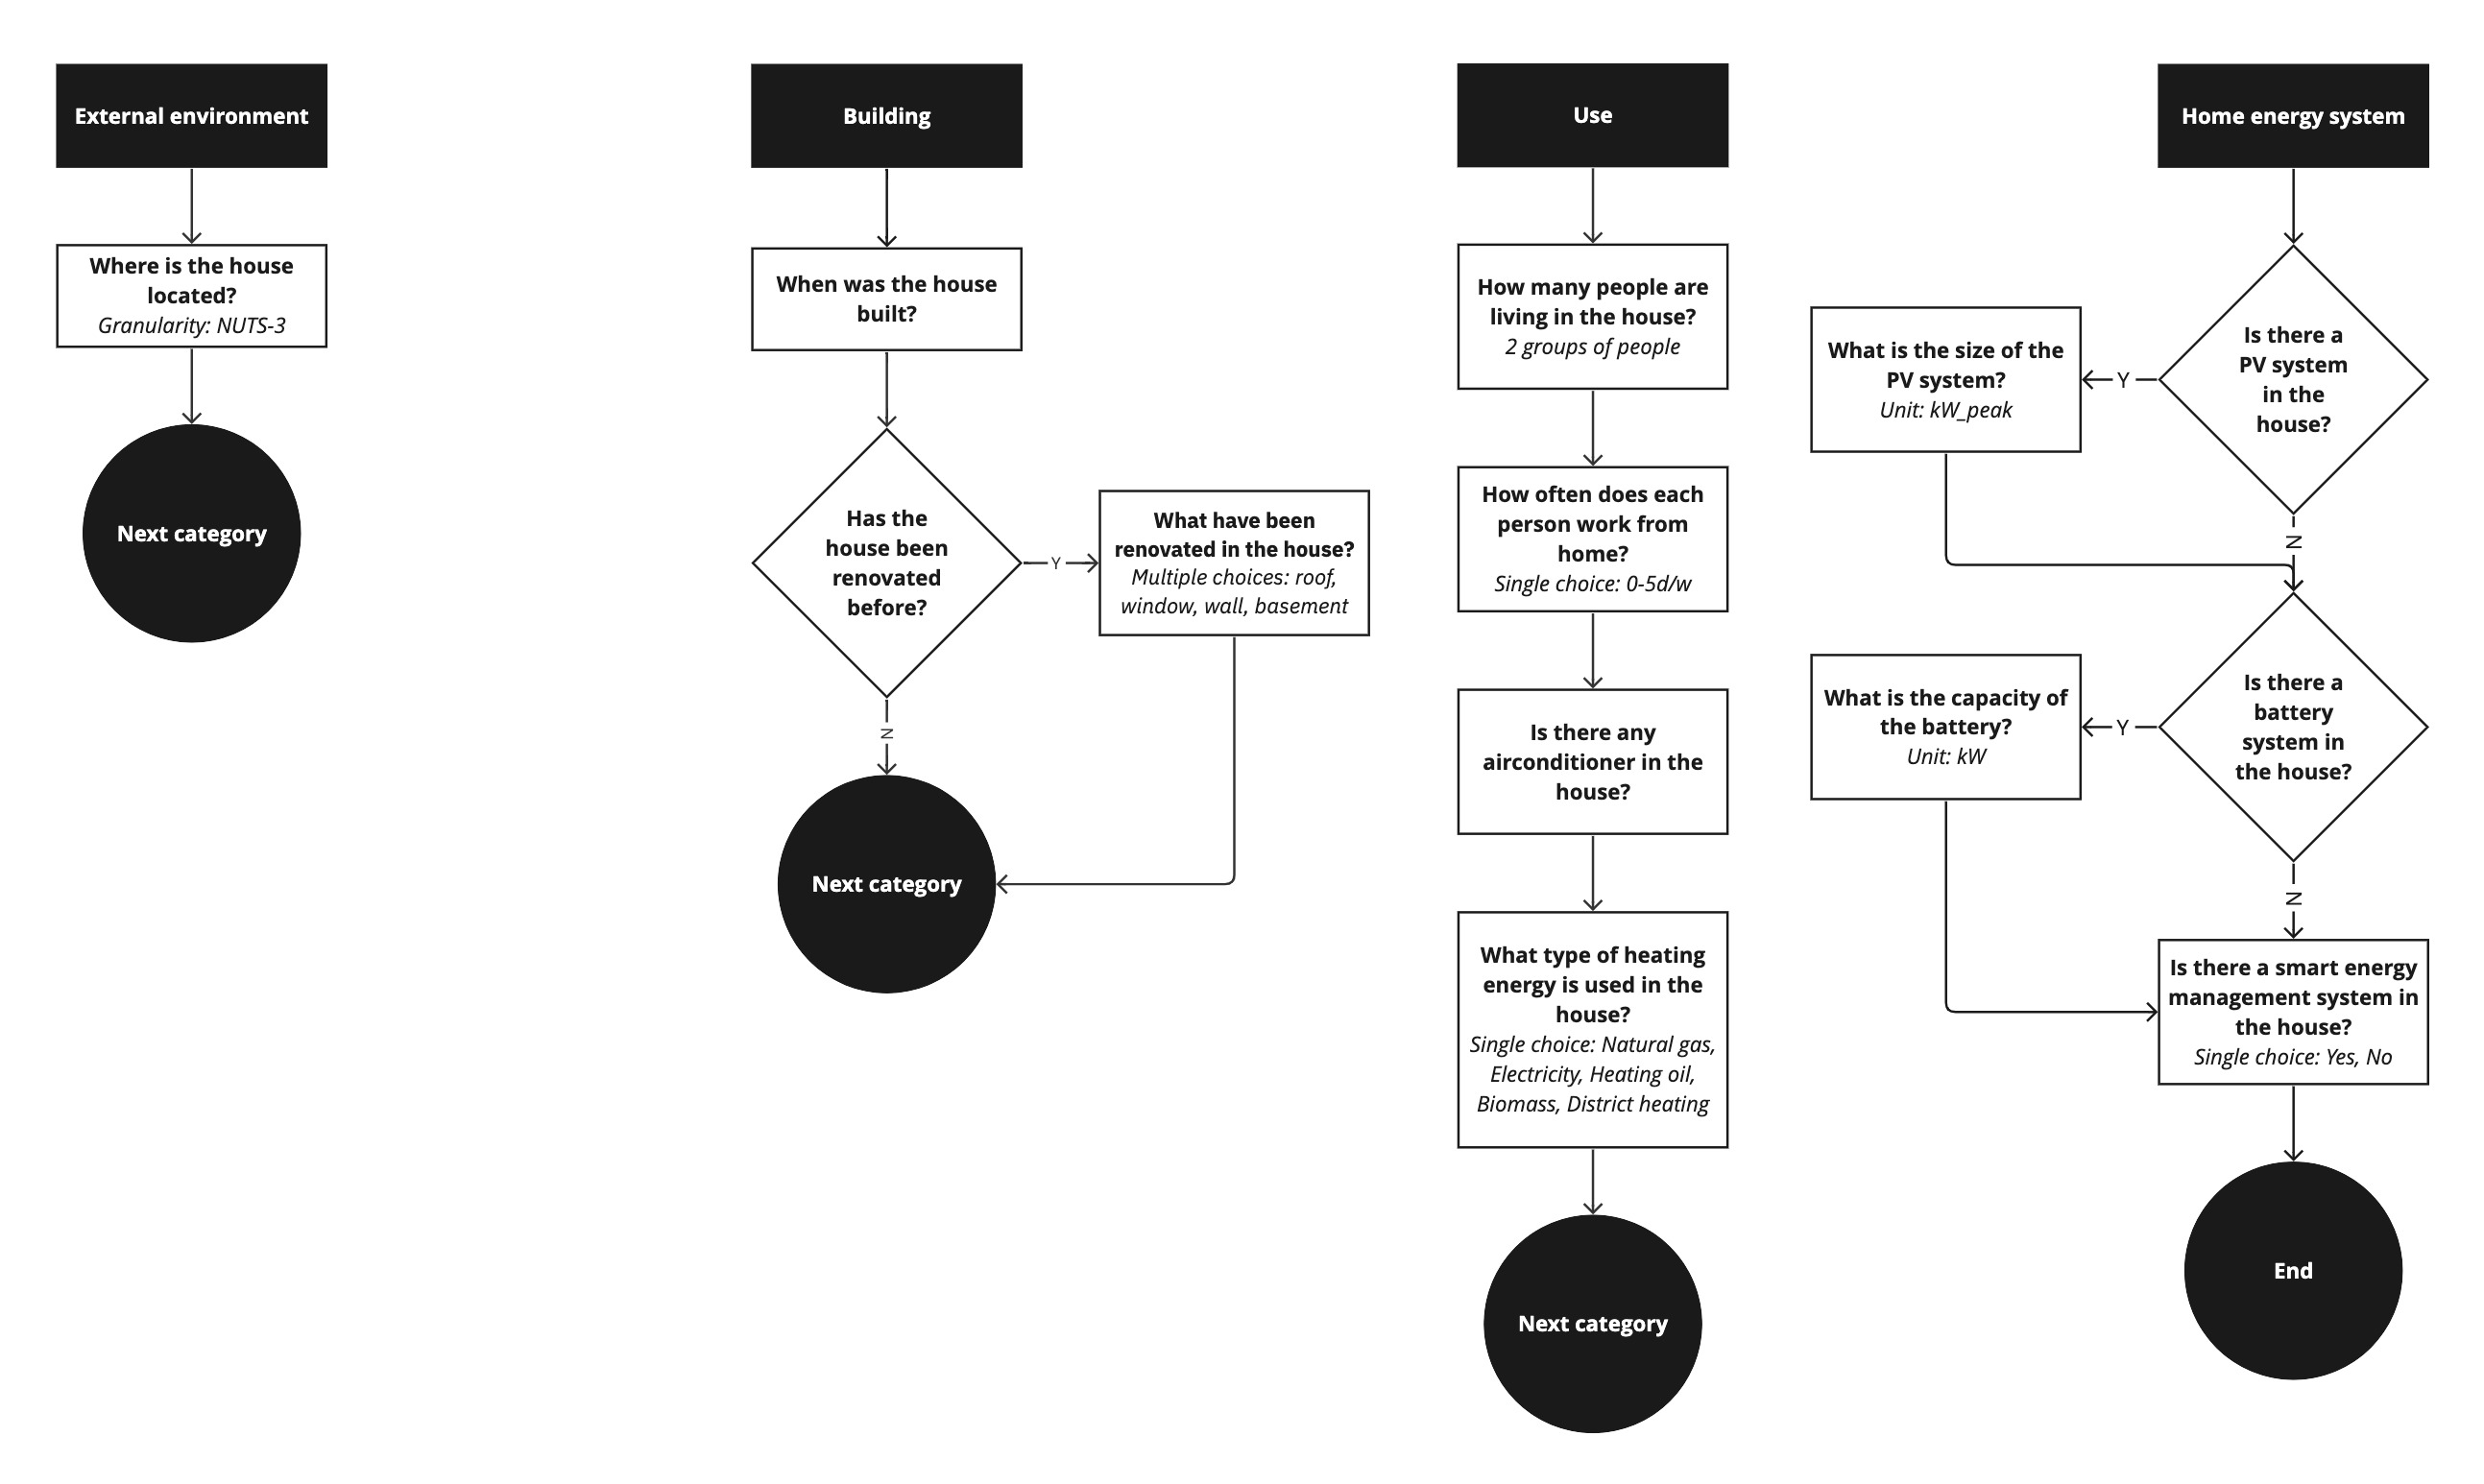
\includegraphics[width=\textwidth]{Images/trees.jpg}
  \caption{Question decision trees}
  \label{fig:trees}
\end{figure}


\section{Output from the recommender}


\subsection{Recommendations}

A sustainable home energy system should prioritise 
\emph{energy-efficiency, reducing dependence on non-renewable fossil fuels, and lowering overall energy costs}. 
All recommendations aligned with these fundamental principles, 
aim to promote sustainable energy practices while also reducing household energy expenditures will be presented to users. 


\subsubsection{Recommendation rules}

The recommendation generation process follows a rule-based approach. 
All recommended technologies either generate renewable energy or exclusively utilise renewable energy sources. 
Additionally, other recommended technologies are selected based on their ability to manage energy usage and improve energy efficiency. 
An overview of the recommended technologies and their functionalities can be found in Table \ref{tab:introduction}.
Furthermore, the system applies each combo to the FLEX models and calculates the associated annual energy bills. 
Only those configurations that result in lower energy bills compared to the user's current situation are recommended. 
This ensures that the recommendations provided to users are cost-effective. 


\subsubsection{Recommendation orders}
The recommendations are categorised into different levels, 
each offering different technology configurations along with their corresponding yearly energy bills. 
The default order of the recommendations follows a prioritisation based on potential cost savings. 
Therefore, the configuration that offers the highest amount of money saved will be listed at the top, followed by the second-best money-saving configuration, and so forth. 
This ordering allows users to easily identify the most financially advantageous options for their energy system.
In addition to the default ordering, users also have the option to select an alternative ordering rule. 
The alternative rule ranks the recommendations based on investment cost, with the configurations requiring the least expenses listed at the top. 
Two distinct ways of ordering options provides users with flexibility, allowing them to prioritise their choices based on their individual financial considerations. 

%The objectives of the recommendation system are multi-fold. 
%Firstly, the system aims to support homeowners in making informed decisions regarding investments in home energy systems. 
%Additionally, the system intends to encourage behavior change among homeowners by promoting the utilization of renewable energy sources. 
%Finally, the recommendation system seeks to continuously refine and improve the accuracy of its predictive model, ensuring that the recommendations provided are up-to-date and effective. 
%By providing users with tailored recommendations, the system aims to facilitate the adoption of energy technologies, ultimately leading to reduced energy demand and associated costs. 
%
%As noted by Karen Palmer et al. \cite{informationgap}, financial considerations are of primary importance to homeowners when making decisions about energy investments. 
%In line with this understanding, the recommendation system places a strong emphasis on providing transparent cost estimates for energy bills as well as recommended home energy system configurations. 
%Additionally, the system seeks to encourage behavior change by providing information and education on climate change and renewable energy sources, aimed at increasing user awareness and understanding of the benefits of sustainable energy practices. 
%To facilitate ongoing improvement and refinement of the recommendation system, a feedback survey button will be incorporated, allowing users to provide both short-term and long-term feedback on the system's performance and recommendations. 


\subsection{Explainability}

Explainability plays a crucial role in establishing trust among users in Recommendation Systems (\gls{rs}), and this principle holds true for our system as well. 
When the system generates recommendations for users, it is important for users to understand why a particular configuration is being recommended to them. 
Explanations aim to bridge this gap by shedding light on the factors that contribute to the recommendation and how they align with the user's preferences (the financial aspect specifically). 


\subsubsection{Explanation}

According to Nunes and Jannach \cite{Nunes2020}, previous studies have identified ten purposes of explanations, including 
\emph{transparency, effectiveness, trust, prersuasiveness, satisfaction, education, scrutability, efficiency, debugging}.
In our case, the explanations provided by the system are intended to serve three purposes: 
\emph{effectiveness, trust, and education}. 
\begin{description}
  \item[Effectiveness] The system aims to support users in making informed decisions by providing the corresponding yearly energy bill. 
    As they can immediately gauge the financial implications and potential cost savings associated with each recommendation. 
  \item[Trust] By offering more detailed simulated energy consumption patterns, users gain a deeper understanding of how the energy bills are calculated in the recommended configurations, 
    thereby building trust and confidence in the accuracy and reliability of the system's outcomes.
  \item[Education] The system utilises explanations as educational tools to offer users valuable insights into the recommended technologies and their impact on energy bills, 
    furthermore, the system can also provide information about the broader context of climate change, helping users understand the larger picture and the importance of sustainable energy practices.
\end{description}


\subsubsection{Exploration}

Beside retrospective explanations, prospective user interfaces can play a significant role in guiding users incrementally toward their goals and enhancing user control and transparency in the recommendation process. 
According to a study by Siepmann and Chatti \cite{Siepmann2023}, such interfaces have the potential to facilitate the development of a more accurate mental model of the decision-making system.
Therefore, in our design, by providing interactive and visual interfaces, users are empowered to actively explore and adjust various configurations of the recommended technologies. 
This level of control allows users to observe and analyse the corresponding simulated results in real-time. 
As users manipulate the configurations, they gain a better understanding of how changes impact the outcomes. 
By making the system's workings visible and allowing users to actively participate, users can develop a clearer mental model of how the system functions and how different choices influence the results. 
This transparency and user empowerment contribute to increased trust and understanding of the decision-making system.


\subsubsection{Levels of explanations}

In addition, a study conducted by Kim et al. \cite{Kim2023} examined the explainability needs of 20 diverse end-users 
and revealed that the level of explainability required varied based on participants' backgrounds in AI and their interests in the domain. 
While there was a general curiosity about AI among participants, only those with a high level of AI expertise or a significant interest in the domain expressed a need for detailed explanations regarding the \gls{rs} system. 
Therefore, it is essential to provide different levels of explanations to accommodate the varying characteristics of users and meet their specific needs. 
\begin{description}
  \item[The first level of explanation] For users who are primarily focused on improving their home energy systems without a deep interest in understanding the underlying system, 
    this level of explanation presents the recommended configurations, specifying the technology products that should be installed or upgraded in their homes. 
    Additionally, it provides information on the corresponding yearly energy bills associated with each configuration. 
    The objective is to ensure that users comprehend the potential benefits of implementing the recommendations. By clearly presenting the recommended configurations and their associated energy bills, users can readily evaluate the potential improvements that can be achieved in terms of energy efficiency and cost savings. 
  \item[The second level of explanation] For users who have doubts about the recommendations and possess a curiosity about how the system operates, 
    besides the first level information, this level of explanation offers insights through generated energy consumption patterns and encourages user exploration to understand the underlying workings of the system. 
    They can observe how different configurations or technology choices impact energy consumption and ultimately influence the calculation of yearly energy bills. 
    By facilitating user interaction and transparency, the system aims to build trust and alleviate doubts, enhancing user confidence in the system's recommendations.
  \item[The third level of explanation] This level of explanation focuses on providing cognitive knowledge to users. 
    It goes beyond the technical aspects of the system and delves into the broader context of environmental protection and sustainability. 
    Users are encouraged to consider the long-term consequences of their energy-related decisions and their role in contributing to a more sustainable future. 
    It aims to raise awareness among users, foster a sense of responsibility, and offer additional information and resources for embracing sustainable practices beyond the immediate recommendations of the system.
\end{description}


\subsubsection{Additional information}

In addition to the aforementioned, there are several other techniques that are considered to further support users in their decision-making process. 
These techniques aim to provide additional information to enhance user understanding, facilitate comparisons, and enable informed choices. 
\begin{description}
  \item[Comparison with current situation] To ensure users can verify the accuracy of our system, we provide a valuable reference point by offering simulated versions of their current energy bill and consumption. 
    This feature allows users to compare the system's simulations with their actual energy usage, enabling them to assess the reliability and accuracy of the recommendations. 
    By presenting users with their simulated current energy bill and consumption, they can directly observe how closely the system's simulations align with their real-life data. 
    This serves as a tangible measure of the system's effectiveness and enhances user confidence in its recommendations. 
    The verification process not only fosters user trust and confidence but also allows us to collect valuable user feedback for continuous improvement.
    By actively seeking user perspectives and incorporating their feedback, we can refine the algorithms and models, ensuring that the recommendation system evolves and remains responsive to users. 
  \item[Technology explanation] a brief explanation (Table \ref{tab:introduction}) of each recommended technology is provided to help users understand their functionalities and how they contribute to energy efficiency. 
    The technology introductions are presented in a clear and straightforward manner, avoiding technical jargon and using language that is easily understandable for users with varying levels of knowledge about energy systems. This ensures that users can quickly grasp the main concepts and functionalities of each technology without feeling overwhelmed by complex technical details.
    It empowers users to make more informed decisions by providing them with the necessary knowledge to assess the relevance and suitability of each technology for their specific energy needs and goals.
    \begin{center}
      \begin{table}[h!]
      \small
          \begin{tabular}{ | p{.20\textwidth} | p{.70\textwidth} | }
            \hline  
            \textbf{Technology} & \textbf{Explanation} \\
            \hline
            \gls{pv} system & A PV system can convert sunlight directly into electricity. \\
            \hline
            Battery system & A battery system can store excess energy generated by solar panels or other renewable sources of energy during the day. \\
            \hline
            \gls{sems} & A Smart Energy Management System (SEMS) can optimise energy usage by adjusting heating and cooling systems, lighting, and other energy-consuming devices to minimise energy waste; and turning off or reducing energy usage during periods of low occupancy or when energy prices are high. \\
            \hline
            \gls{hp}&  A heat pump is a device that transfers heat from one place to another, providing both heating and cooling for spaces. \\
            \hline
            Hot water tank & A hot water tank is a device used to store domestic hot water for use in homes. The hot water in the tank can be used in sinks, showers, or appliances. \\
            \hline
            Space heating tank & A space heating tank is a device used to store hot water to provide heat to interior spaces in homes. \\
            \hline
            Building renovation & Building renovation can have a significant impact on improving home energy efficiency performance by reducing the amount of energy needed to heat, cool, and operate a home. \\
            \hline
          \end{tabular}
      \caption{Brief introduciton of each technology}
      \label{tab:introduction}
      \end{table}
    \end{center}
  \item[Investment costs] The consideration of supplementary information pertinent to users' investment decisions holds significance. 
    Hence, we endeavor to furnish users with additional information regarding technology costs. 
    However, it is imperative to acknowledge that various brands exhibit divergent pricing structures, and the performance or size variations of individual technologies directly influence their corresponding costs. 
    In light of this, we present users with a range of costs associated with each technology, aiming to facilitate their decision-making process by fostering informed choices. 
    The specific cost ranges are presented in the Table \ref{tab:investments}.
    \begin{center}
      \begin{table}[h!]
      \small
          \begin{tabular}{ | p{.20\textwidth} | p{.15\textwidth}  p{.15\textwidth}  p{.15\textwidth}  p{.15\textwidth} | }
              \hline
              Technology & \multicolumn{4}{ c | }{Cost (\euro{})} \\
               & Lowest & Highest & Installation & Maintenance \\
              \hline
              \gls{pv} system & \SI[per-mode=symbol,bracket-unit-denominator = false]{1957,68}{\per\kW}p & \SI[per-mode=symbol,bracket-unit-denominator = false]{2231,76}{\per\kW}p & included & 0 \\
              Battery system & \SI[per-mode=symbol,sticky-per,bracket-unit-denominator = false]{790,80}{\per\kWh}  & \SI[per-mode=symbol,sticky-per,bracket-unit-denominator = false]{2520,00}{\per\kWh} & included & 0 \\
              \gls{sems} & / & 1516,11 & 379,03 & 0 \\
              \gls{hp}& \SI[per-mode=symbol,bracket-unit-denominator = false]{432,15}{\per\kW} & \SI[per-mode=symbol,bracket-unit-denominator = false]{2370,31}{\per\kW} & included & 0 \\
              Hot water tank & 1 & 1 & 1 & 0 \\
              Space heating tank & 1 & 1 & 1 & 0 \\
              Air conditioner & 1 & 1 & 1 & 0 \\
              Basement renovation & \SI[per-mode=symbol]{132,12}{\per\metre\squared} & \SI[per-mode=symbol]{157,64}{\per\metre\squared} & included & 0 \\
              Roof renovation & \SI[per-mode=symbol]{40,95}{\per\metre\squared} & \SI[per-mode=symbol]{409,38}{\per\metre\squared} & included & 0 \\
              Wall renovation & \SI[per-mode=symbol]{67,57}{\per\metre\squared} & \SI[per-mode=symbol]{408,93}{\per\metre\squared} & included & 0 \\
              Window renovation & \SI[per-mode=symbol]{364,63}{\per\metre\squared} & \SI[per-mode=symbol]{958,92}{\per\metre\squared} & included & 0 \\
              \hline
          \end{tabular}
      \caption{Investment costs of different technologies}
      \label{tab:investments}
      \end{table}
  \end{center}
\end{description}

%In order to provide more comprehensive and understandable recommendations, we have chosen to explain our recommendations from multiple perspectives beyond just cost estimates. 
%Specifically, we have identified 4 key objectives, including \emph{trust, effectiveness, education, and debugging}, as key aspects to incorporate into our explanations. 
%\emph{Trust}, we build trust with our users by using reliable data sources and providing transparent services. 
%\emph{Effectiveness}, we strive to enhance the effectiveness of our service by offering recommendations that could actually benefit users economically. 
%\emph{Education}, we seek to educate our users on the importance of environmental protection by sharing relevant knowledge and insights. 
%\emph{De-bugging}, we value user feedback as an important tool for identifying and resolving any issues or bugs in our system, allowing us to continuously improve and refine our service.
%The reasons for offering such explanations are to familiarise users with these technologies, establish accountability in the decision-making process, and encourage a shift towards environmentally conscious behaviour.
%By incorporating these concepts into our explanations, we aim to provide recommendations that are transparent, trustworthy, understandable, and user-centred. 
%
%Our recommendation system employs a three-level explainability framework to enhance user understanding of the recommended home energy system configurations. 
%At the first level, the system provides an explanation in terms of the expected energy bill for the household. 
%At the second level, the system offers a behavioural explanation of energy consumption patterns and the factors driving them. 
%Finally, at the third level, the system aims to increase users' awareness and understanding of renewable energy and environmental protection.
%
%Furthermore, the explanation is divided into three layers. 
%At the first layer, users are provided with a comprehensive summary of their current energy consumption patterns. 
%At the second layer, users are introduced to the various functionalities and benefits of the recommended energy technologies, including cost-saving potential and environmental impact. 
%Finally, at the last layer, users are presented with simulated energy demand and supply data, allowing them to see the potential energy savings that could result from adopting the recommended configurations. 
%
%Through the implementation of a comprehensive approach to explainability, our objective is to offer users an overview of energy technologies, enabling them to gain insight into their energy consumption patterns and to recognize the advantages of shifting towards more sustainable energy systems.


\subsubsection{Presetation}

Both Natural language (\gls{nl}) and Information visualisation (\gls{iv}) techniques are used to serve different purposes and enhance the overall clarity and effectiveness of conveying information to users. 
\gls{nl} explanations, in the form of textual descriptions, are utilised to provide detailed information about technology functionalities and costs. 
Charts are employed to present energy consumption data in a visual format. 
Visualising energy consumption data of each sector using charts helps to simplify complex information, enabling users to grasp patterns and comparisons more easily. 
Users can observe the relative contributions of different sectors, identify areas of high or low energy consumption, and explore alternative scenarios or configurations. 


\section{Medium}

At present, the service is designed as a one-time interaction where users receive recommendations and may not revisit the system in the near future. 
Meanwhile, the explanations provided can be presented in a highly detailed manner, as users have the opportunity to carefully read and understand the information. 
The interactive nature of the system allows users to compare complex data and explore different configurations. 
A larger screen offers a more comfortable viewing experience, therefore, the current focus is on desktop or larger screens.
However, considering the prevalent use of smartphones in today's society, it is important to acknowledge the need for a mobile-friendly version of the service. 


\section{Interfaces}

In this chapter, several key interfaces are explained, providing an overview of the important pages and features of the system. 
While not all pages are covered, the focus is on highlighting the interfaces that play a significant role in the user experience and decision-making process. 


\subsection*{Homepage}

The homepage (Figure \ref{fig:homepage}) of the website serves the purpose of informing participants about the functionality and process of the service. 
Several factors related to usability are considered in the design and content of the home page:
\begin{description}
  \item[Purpose introduction] The homepage should clearly communicate the purpose of the service, highlighting its main objective and benefits for participants, in order to help users understand the core function and value proposition of the website.
  \item[Explanation of steps] A 2-step explanation is provided to guide users through the process of using the service even before they begin, this is to ensure that users are mentally prepared for the service and have a clear roadmap to follow. 
  \item[A time indicator] The estimated time required to complete the questionnaire is provided to users as a feature to mentally prepare them for the task at hand. By indicating the expected time commitment, users can have a better understanding of the anticipated duration of their engagement with the system. 
  \item[Data privacy information] Users are informed about the data handling practices and security measures implemented by the website. Additionally, users also have the opportunity to delve deeper into the specifics of data handling practices by accessing more detailed information. The privacy policy can be found in Appendix \ref{appendix:privacy}. 
  \item[Involvement of organisations] The homepage introduces the relevant organisations involved in the development and operation of the service to establish credibility in the reliability and expertise of the system.
  \item[Contact details] Email addresseses is provided to allow participants to reach out for support, clarification, or any other inquiries they may have.
  \item[Language options] The service offers language options in both English and German to cater to a broader audience in Europe.
\end{description}
\begin{figure}[h!]
  \centering
  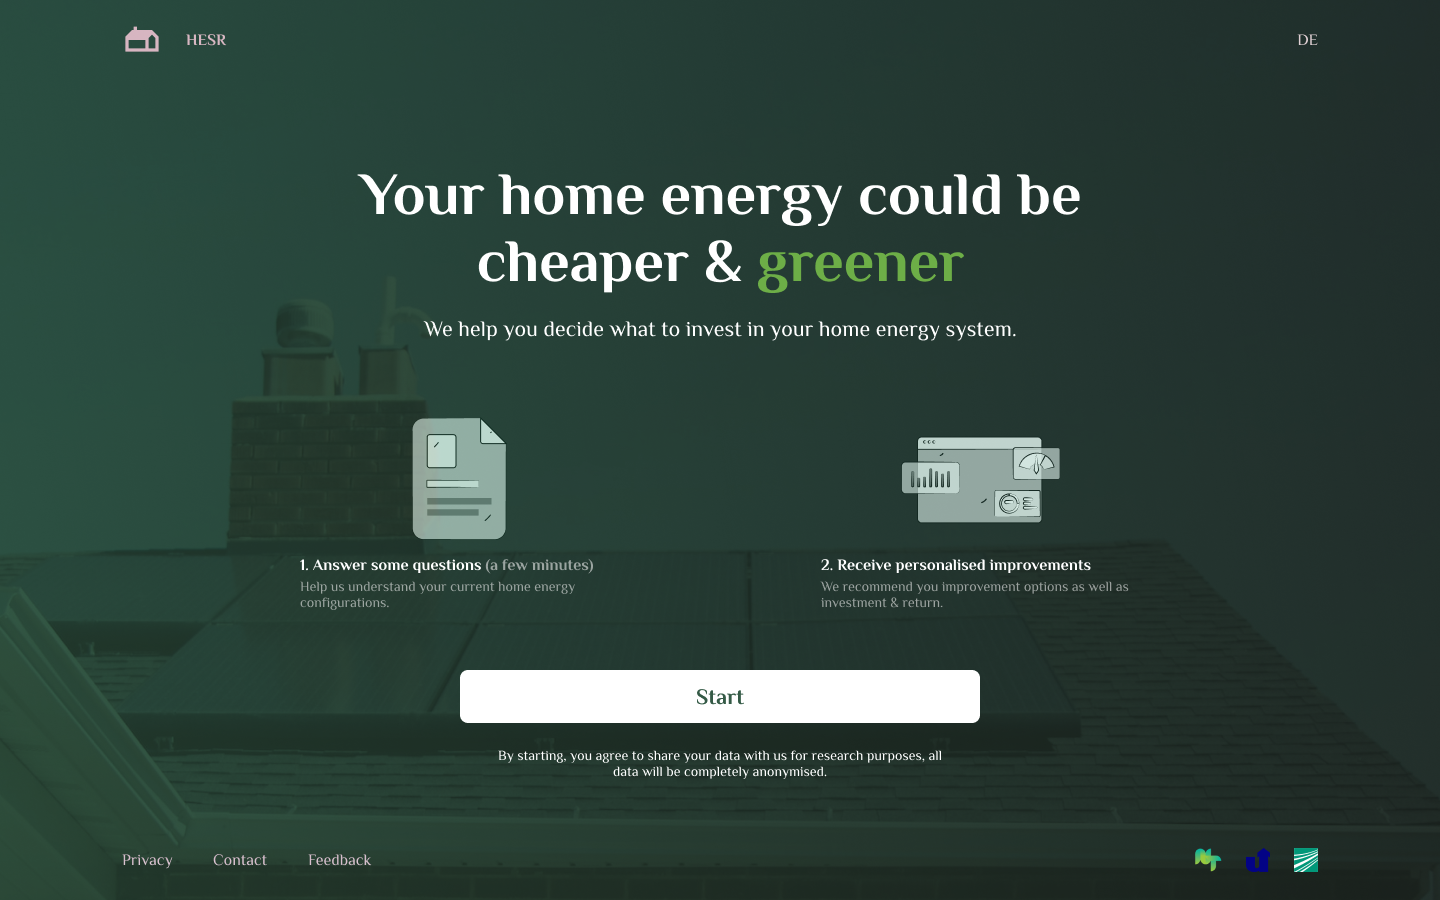
\includegraphics[width=\textwidth]{Images/welcome.png}
  \caption{Homepage}
  \label{fig:homepage}
\end{figure}


%To facilitate user understanding of the recommended home energy system configurations and associated costs, our recommendation system will employ a visual and natural language explanation interface. 
%Specifically, an interactive visualization tool will be implemented to enable users to explore and compare different energy system configurations in terms of energy consumption patterns and costs. 
%Additionally, natural language explanations will be provided to further enhance user understanding and engagement with the recommended configurations. 


\subsection*{Questionnaire}

The questionnaire page (Figure \ref{fig:question}) is specifically designed to collect information pertaining to the household's current energy demand and supply-related factors. 
Its purpose is to gather comprehensive data in order to construct a detailed household profile.
Several usability factors are taken into account to enhance user experience on this page:
\begin{description}
  \item[One question at a time] To present one question at a time, ensuring that users understand precisely what information is being requested from them. 
    Users can focus their attention on each individual question without feeling overwhelmed by a large set of inquiries, which allows for better comprehension and reduces the risk of confusion or misunderstanding. 
  \item[Question categorisation] Each question is assigned a relevant category to provide context to users.
  \item[Transparent process] The page outlines the overall process, indicating the number of categories involved.
  \item[Detailed explanations] For unfamiliar or complex concepts, the page offers more detailed explanations to provide users with a better understanding.
  \item["I Don't Know" option] Users are provided with an option to select "I don't know" if they are unsure about a particular question. 
  \item[Return and edit] The page allows users to easily navigate back to the previous page and make changes if they need to modify their answers. 
\end{description}
\begin{figure}[h!]
  \centering
  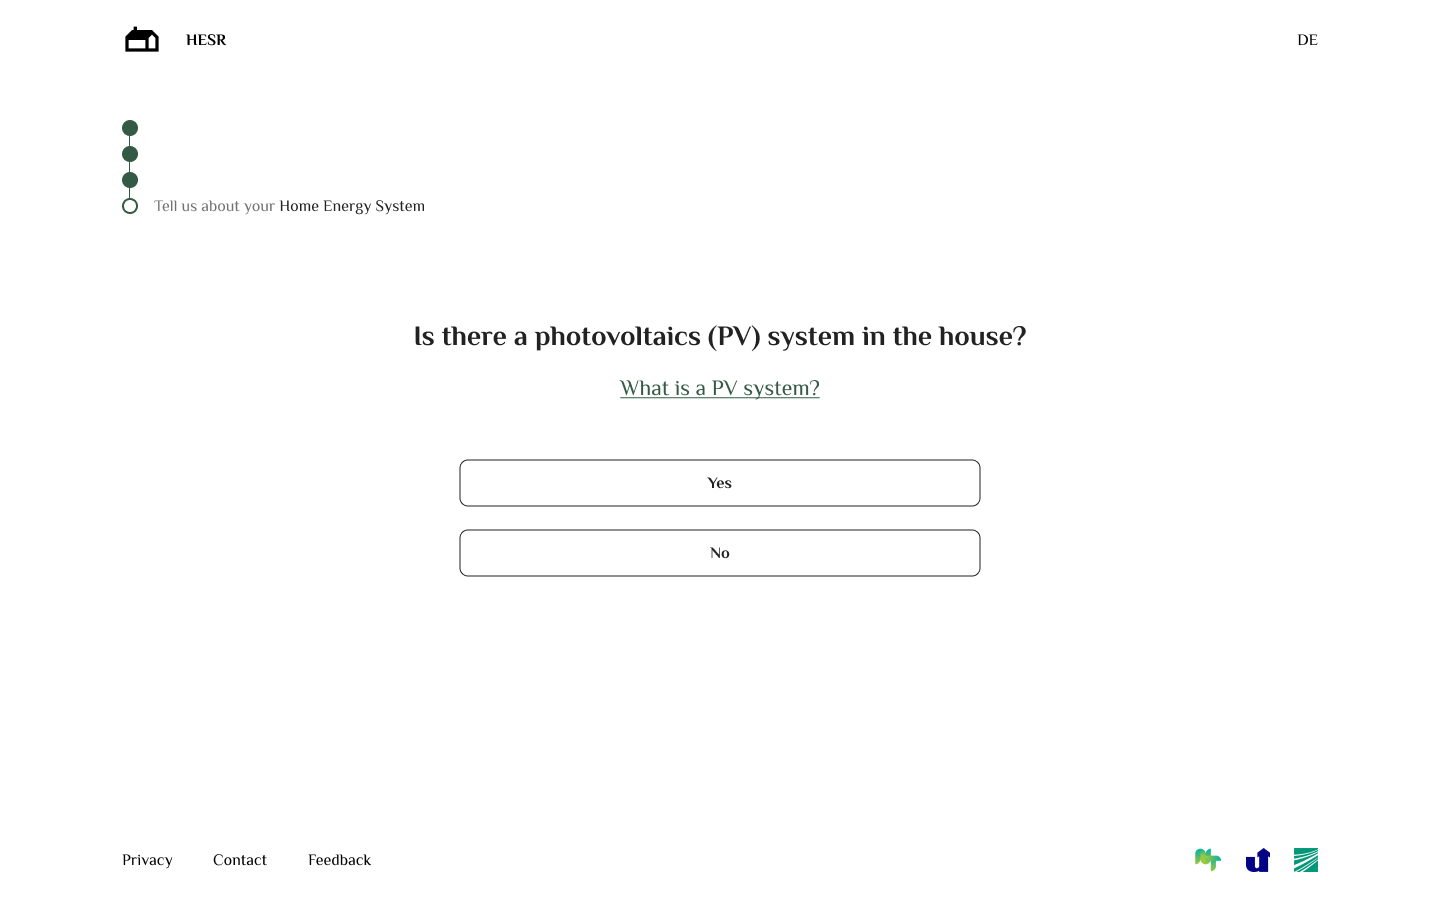
\includegraphics[width=\textwidth]{Images/question.png}
  \caption{Questionnaire}
  \label{fig:question}
\end{figure}


\subsection*{Recommendation}

The recommendation page (Figure \ref{fig:recommendation} and \ref{fig:recommendation_null}) serves as a crucial component of the system, aiming to inform users about the available home energy system options that can potentially lower future energy costs and improve energy efficiency. 
The page provides clear and simple explanations (annual energy costs) behind each recommendation.
To ensure usability and meet user needs, the recommendation page incorporates the following features:
\begin{description}
  \item[List of recommendations] The page presents all the recommended options, or in some cases, informs users if no specific recommendation is available. 
  \item[Estimated current energy bill]  Users are provided with an estimated current energy bill, allowing them to compare their existing energy costs with the potential savings offered by the recommended options. This provides a tangible reference point for users to assess the financial impact of the recommendations.
  \item[Flexible orders] The system allows for different ways of presenting the recommendations. 
  \item[First level explanation] Each recommended option is accompanied by specific information regarding the potential financial benefits it offers, including money saved and the projected annual energy bills. 
  \item[Allow for detailed sxplanations] For users who seek more in-depth information, the recommendations page offers the option to access more detailed explanations. 
\end{description}
\begin{figure}[h!]
  \centering
  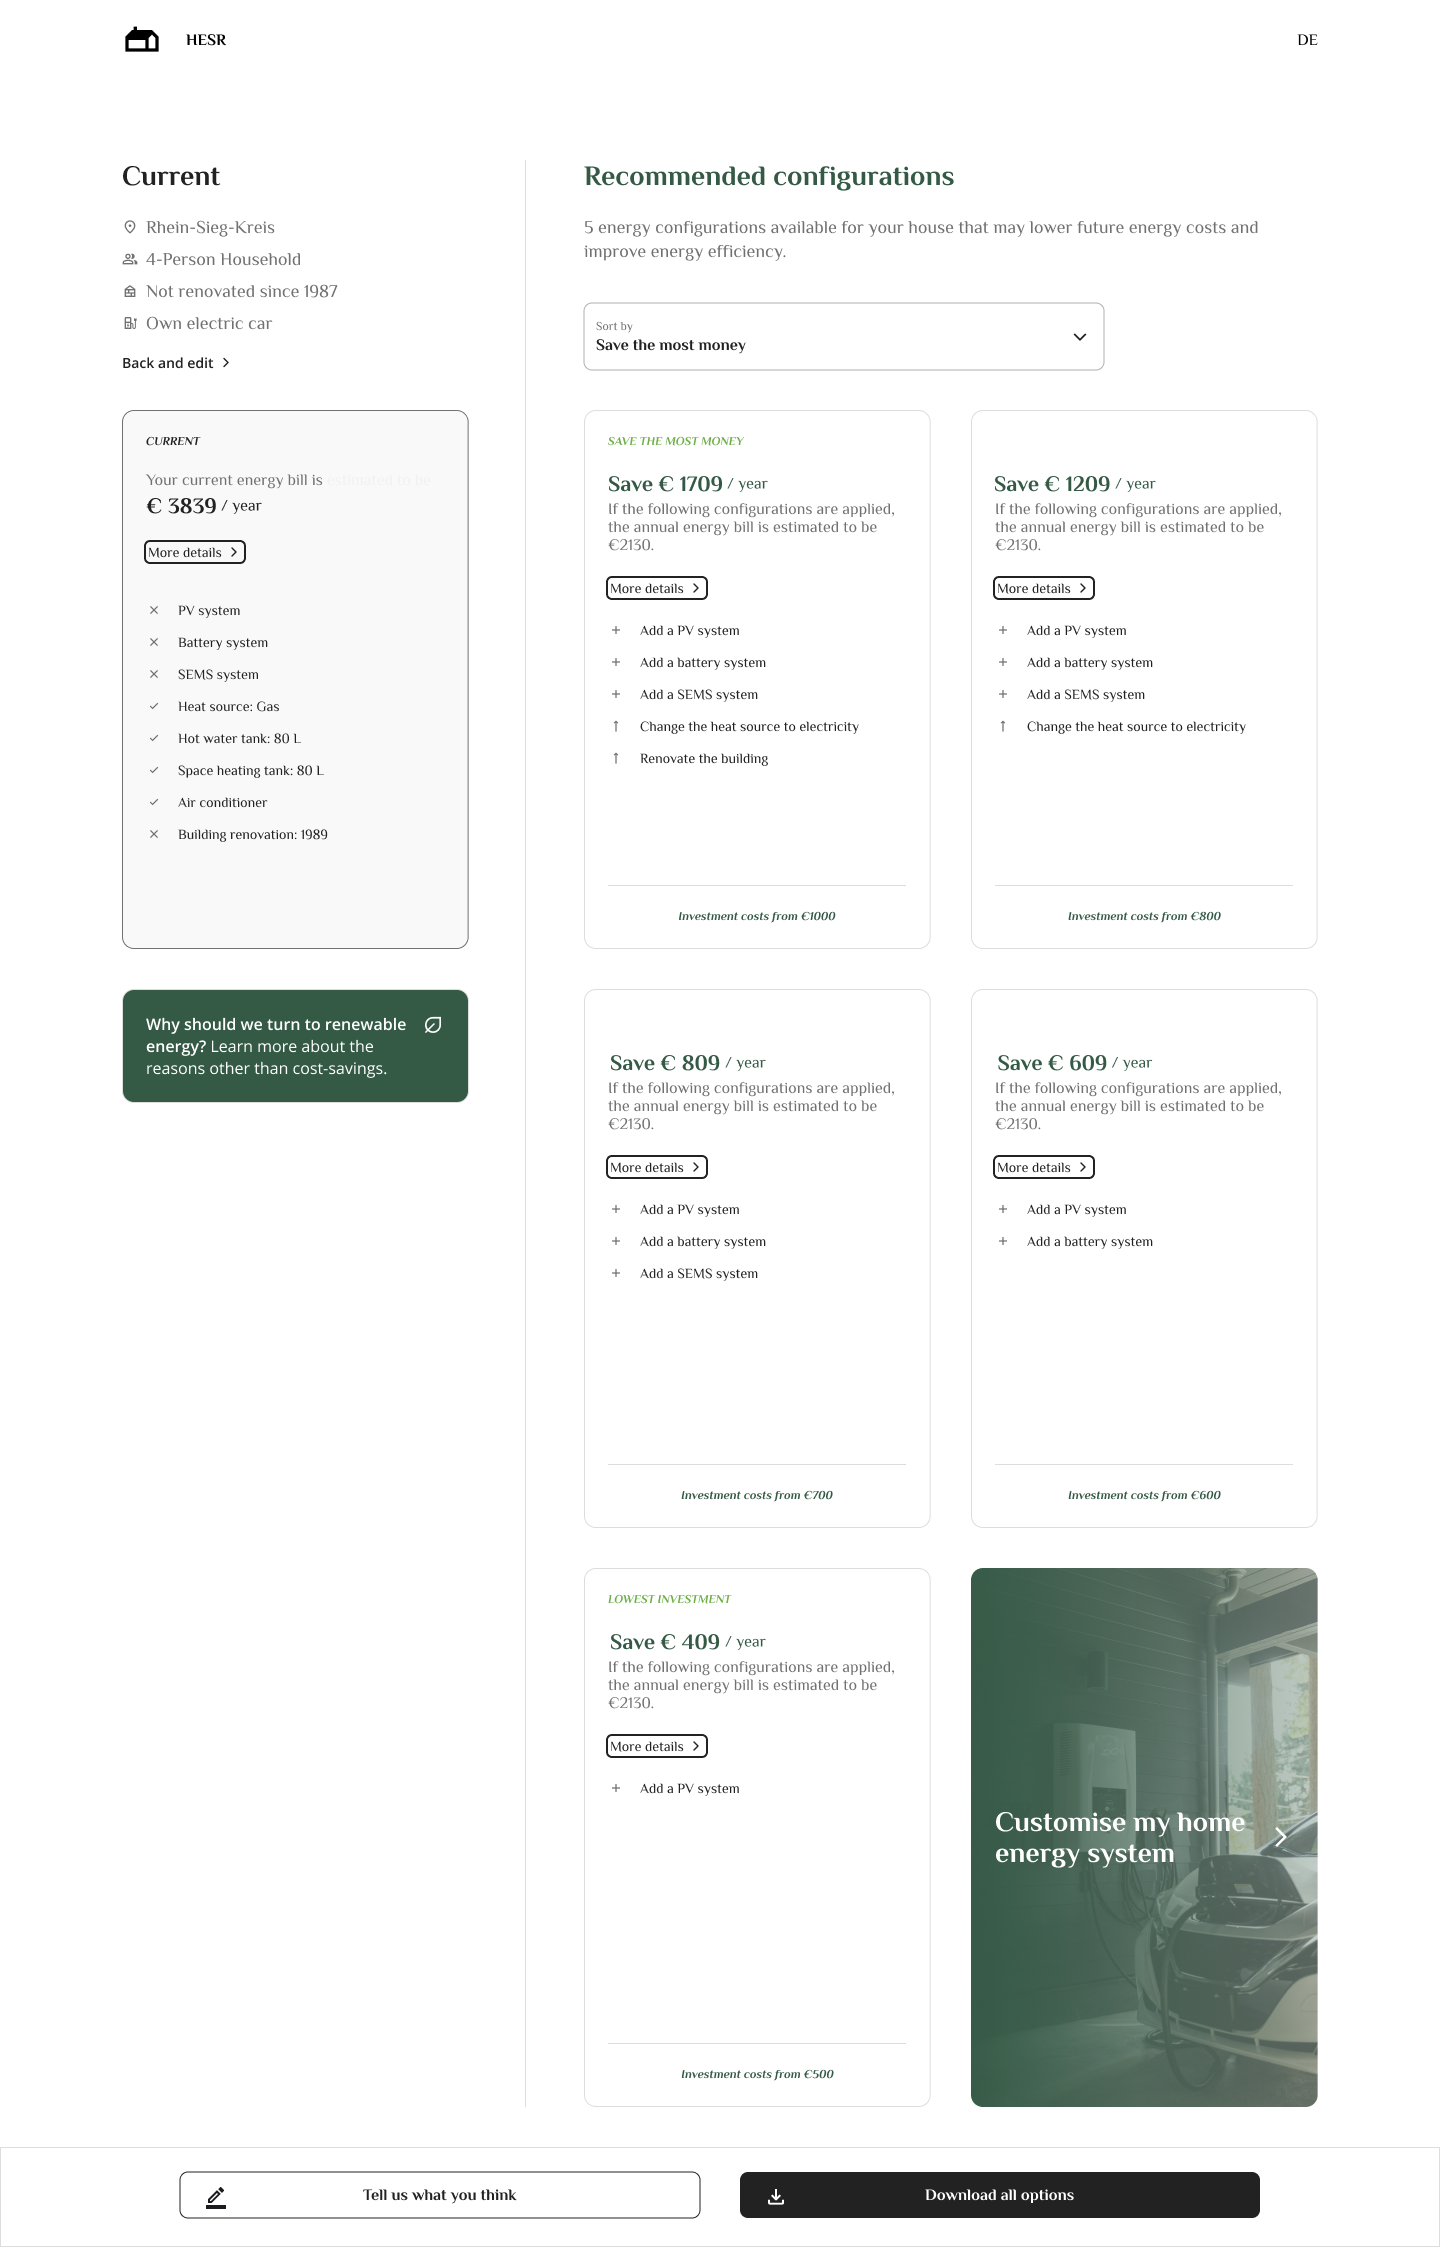
\includegraphics[width=\textwidth]{Images/recommendation.png}
  \caption{With recommendations}
  \label{fig:recommendation}
\end{figure}
\begin{figure}[h!]
  \centering
  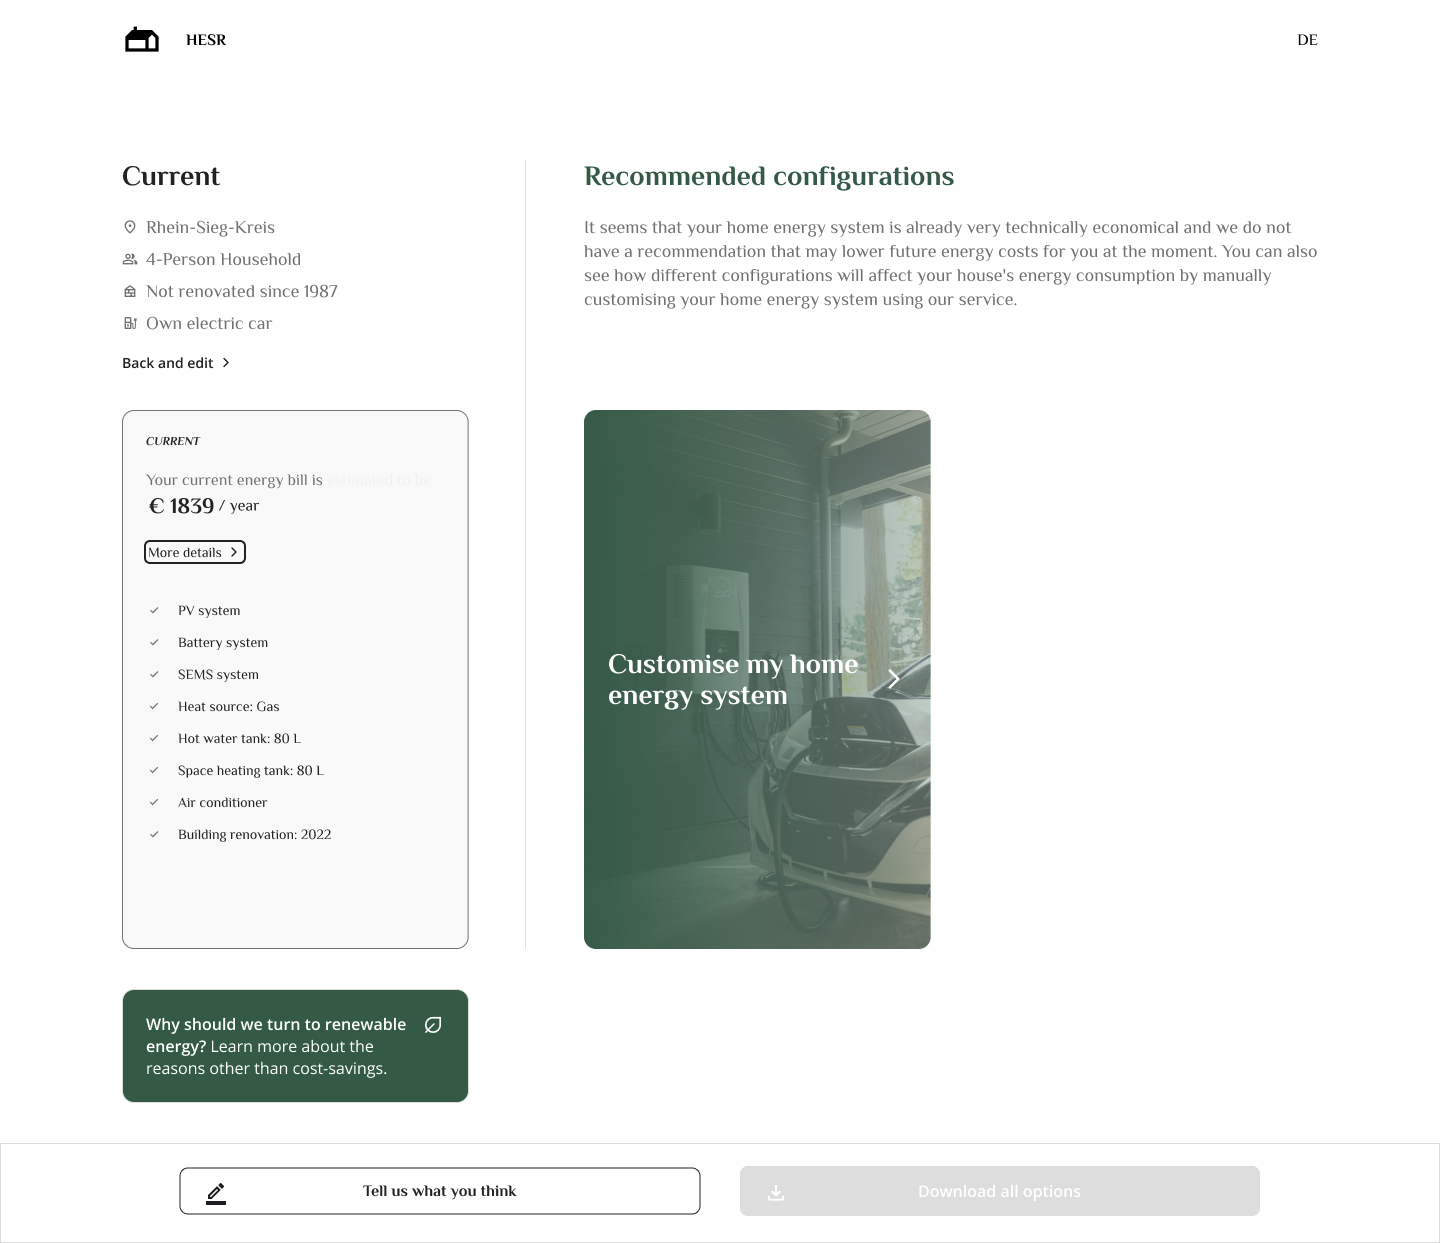
\includegraphics[width=\textwidth]{Images/recommendation_null.png}
  \caption{No recommendation}
  \label{fig:recommendation_null}
\end{figure}


\subsection*{Simulation}

The simulation page (\ref{fig:explanation}) aims to provide users with more detailed explanations about the recommended options.
\begin{description}
  \item[Data visualisation] It utilises data visualization techniques to present information in a visually engaging and easily understandable format.
  \item[Comparison] The simulation page allows users to compare the recommended options with their current configuration using visualised data, making it easier to understand the differences in energy consumption and demand. 
    The comparison enhances users' understanding of the disparities between the recommended options and their current configuration, enabling them to assess the potential benefits. 
  \item[Exploration] The simulation page enables users to make adjustments to the recommended options. 
    Users can modify various parameters, such as the system size, or technology configurations, and recalculate the results accordingly. 
    This interactive functionality empowers users to explore different scenarios and understand how their choices affect the projected outcomes. 
\end{description}
\begin{figure}[h!]
  \centering
  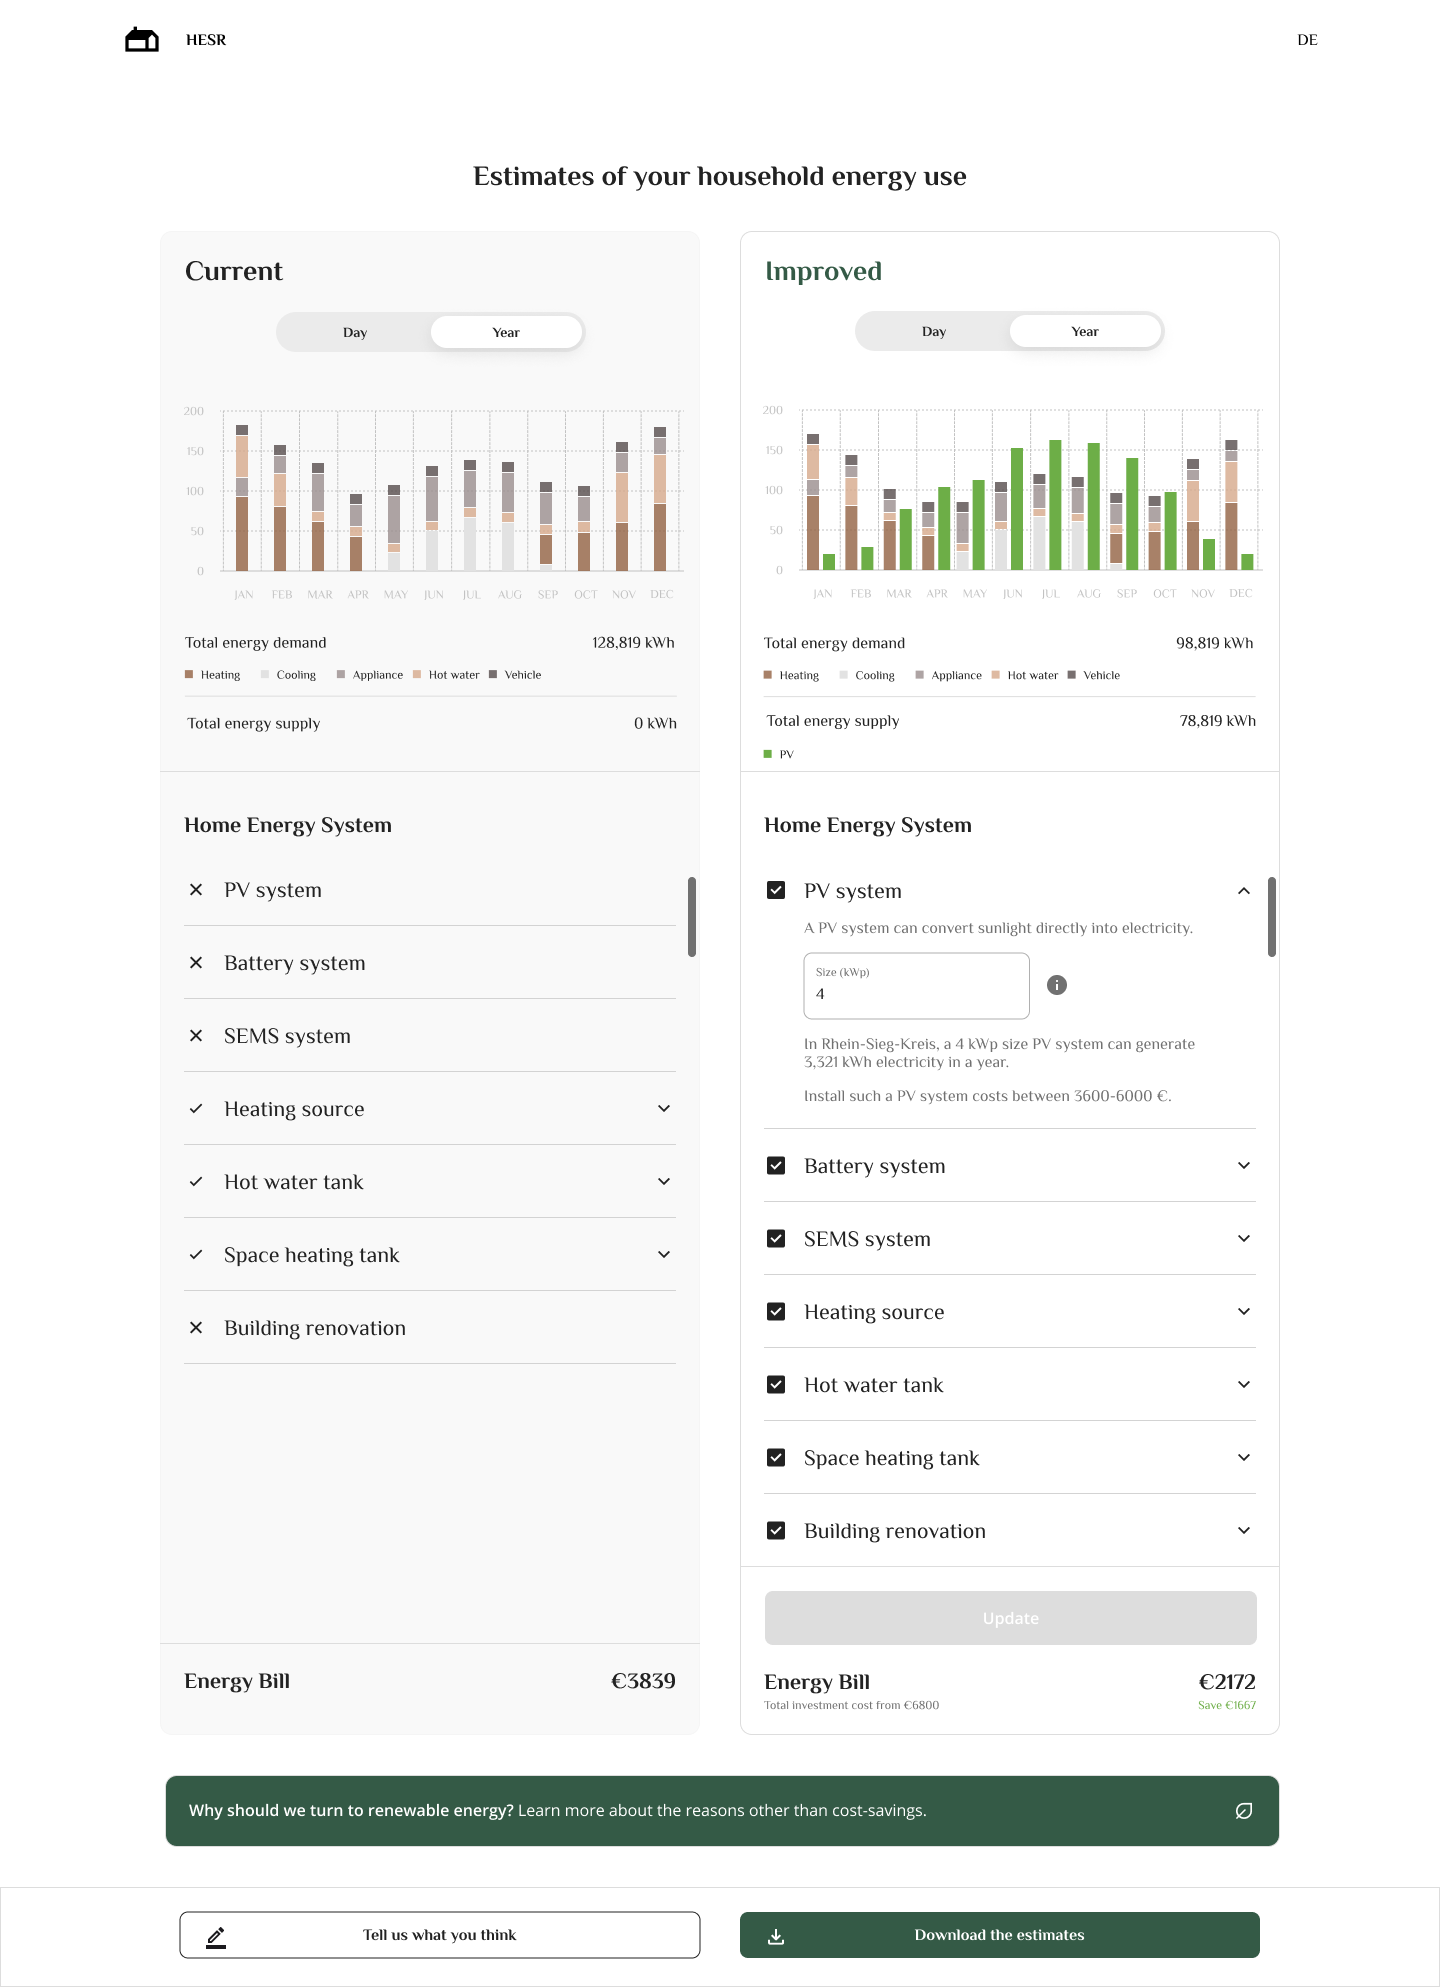
\includegraphics[width=\textwidth]{Images/explanation.png}
  \caption{Simulation page}
  \label{fig:explanation}
\end{figure}